%\begin{comment}
\chapter{Flux d'exécution}
\section{Introduction}
Dans cette annexe, nous allons parler du flux d'exécution d'une requête du client dans le serveur en partant du client jusqu'à la base de données et en revenant pour envoyer une réponse.
\section{Flux d'exécution d'une requête client}
Notre application est divisé en deux parties, la première étant la partie front office implémentée avec AngularJS, et la seconde est la partie back office qui est implémentée avec le framework Spring. Si le client demande l'accès à une certaine information, l'information sera livré comme suit:\\

\begin{enumerate}
    \item AngularJS envoi une requête HTTP au service Rest.
    \item Le service Rest fait appel à une fonction "getResult()" par exemple par l'intermédiaire d'une interface IMetier.
    \item La classe Metier, qui implémente les méthodes de cette dernière, fait appel à une fonction qu'on va appeler "getData()" par l'intermédiaire d'une interface IDAO.
    \item La classe DAO, qui implémente les méthodes de cette dernière, envoi une requête SQL Select spécifique à la donnée demandé à la base de données Oracle qui contient les données de l'application Jira.
    \item La base de données Jira renvoi une réponse contenant la donnée demandé à la classe DAO.
    \item La classe DAO instancie un objet spécifique à la donnée demandé qu'on va appelé "DataModel" puis elle le renvoi à la classe Metier.
    \item La classe Metier fait le mapping entre l'objet DataModel et un objet "DataEntity" puis elle le renvoi à la classe qui implémente notre service Rest.
    \item Le service Rest renvoi alors l'objet DataEntity comme réponse à la requête HTTP provenant du client AngularJS.
    \item AngularJS affiche alors le résultat de la requête.\\
\end{enumerate}

\begin{figure}[H]
  \centering
  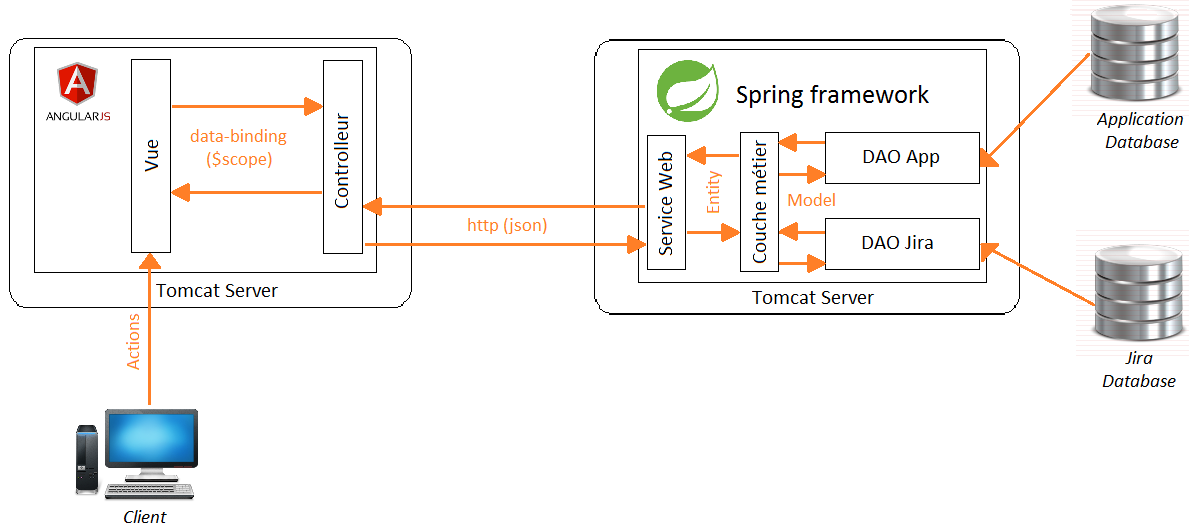
\includegraphics[scale=0.55]{figures/architecture.png}
  \caption{Architecture de l'application}
  \label{code_Architecture}
\end{figure}

\section{Conclusion}
Dans cette annexe, nous avons parlé du flux d'exécution d'une requête du client dans le serveur en partant du client jusqu'à la base de données et en revenant pour envoyer une réponse.
%\end{comment}
